\iffalse
\documentclass[journal,12pt,twocolumn]{IEEEtran}
\usepackage{setspace}
\usepackage{gensymb}
\usepackage{xcolor}
\usepackage{caption}
\singlespacing
\usepackage{siunitx}
\usepackage[cmex10]{amsmath}
\usepackage{mathtools}
\usepackage{hyperref}
\usepackage{amsthm}
\usepackage{mathrsfs}
\usepackage{txfonts}
\usepackage{stfloats}
\usepackage{cite}
\usepackage{cases}
\usepackage{subfig}
\usepackage{longtable}
\usepackage{multirow}
\usepackage{enumitem}
\usepackage{bm}
\usepackage{mathtools}
\usepackage{listings}
\usepackage{tikz}
\usetikzlibrary{shapes,arrows,positioning}
\usepackage{circuitikz}
\renewcommand{\vec}[1]{\boldsymbol{\mathbf{#1}}}
\DeclareMathOperator*{\Res}{Res}
\renewcommand\thesection{\arabic{section}}
\renewcommand\thesubsection{\thesection.\arabic{subsection}}
\renewcommand\thesubsubsection{\thesubsection.\arabic{subsubsection}}

\renewcommand\thesectiondis{\arabic{section}}
\renewcommand\thesubsectiondis{\thesectiondis.\arabic{subsection}}
\renewcommand\thesubsubsectiondis{\thesubsectiondis.\arabic{subsubsection}}
\hyphenation{op-tical net-works semi-conduc-tor}

\lstset{
language=Python,
frame=single, 
breaklines=true,
columns=fullflexible
}
\begin{document}
\theoremstyle{definition}
\newtheorem{theorem}{Theorem}[section]
\newtheorem{problem}{Problem}
\newtheorem{proposition}{Proposition}[section]
\newtheorem{lemma}{Lemma}
\newtheorem{corollary}[theorem]{Corollary}
\newtheorem{example}{Example}[section]
\newtheorem{definition}{Definition}[section]
\newcommand{\BEQA}{\begin{eqnarray}}
\newcommand{\EEQA}{\end{eqnarray}}
\newcommand{\define}{\stackrel{\triangle}{=}}
\newcommand{\myvec}[1]{\ensuremath{\begin{pmatrix}#1\end{pmatrix}}}
\newcommand{\mydet}[1]{\ensuremath{\begin{vmatrix}#1\end{vmatrix}}}
\bibliographystyle{IEEEtran}
\providecommand{\nCr}[2]{\,^{#1}C_{#2}} % nCr
\providecommand{\nPr}[2]{\,^{#1}P_{#2}} % nPr
\providecommand{\mbf}{\mathbf}
\providecommand{\pr}[1]{\ensuremath{\Pr\left(#1\right)}}
\providecommand{\chr}[1]{\ensuremath{\textrm{char}\left(#1\right)}}
\providecommand{\qfunc}[1]{\ensuremath{Q\left(#1\right)}}
\providecommand{\sbrak}[1]{\ensuremath{{}\left[#1\right]}}
\providecommand{\lsbrak}[1]{\ensuremath{{}\left[#1\right.}}
\providecommand{\rsbrak}[1]{\ensuremath{{}\left.#1\right]}}
\providecommand{\brak}[1]{\ensuremath{\left(#1\right)}}
\providecommand{\lbrak}[1]{\ensuremath{\left(#1\right.}}
\providecommand{\rbrak}[1]{\ensuremath{\left.#1\right)}}
\providecommand{\cbrak}[1]{\ensuremath{\left\{#1\right\}}}
\providecommand{\lcbrak}[1]{\ensuremath{\left\{#1\right.}}
\providecommand{\rcbrak}[1]{\ensuremath{\left.#1\right\}}}
\theoremstyle{remark}
\newtheorem{rem}{Remark}
\newcommand{\sgn}{\mathop{\mathrm{sgn}}}
\newcommand{\rect}{\mathop{\mathrm{rect}}}
\newcommand{\sinc}{\mathop{\mathrm{sinc}}}
\providecommand{\abs}[1]{\left\vert#1\right\vert}
\providecommand{\res}[1]{\Res\displaylimits_{#1}} 
\providecommand{\norm}[1]{\left\Vert#1\right\Vert}
\providecommand{\mtx}[1]{\mathbf{#1}}
\providecommand{\mean}[1]{E\left[ #1 \right]}
\providecommand{\fourier}{\overset{\mathcal{F}}{ \rightleftharpoons}}
\providecommand{\ztrans}{\overset{\mathcal{Z}}{ \rightleftharpoons}}
\providecommand{\system}[1]{\overset{\mathcal{#1}}{ \longleftrightarrow}}
\newcommand{\solution}{\noindent \textbf{Solution: }}
\providecommand{\dec}[2]{\ensuremath{\overset{#1}{\underset{#2}{\gtrless}}}}
\let\StandardTheFigure\thefigure
\def\putbox#1#2#3{\makebox[0in][l]{\makebox[#1][l]{}\raisebox{\baselineskip}[0in][0in]{\raisebox{#2}[0in][0in]{#3}}}}
     \def\rightbox#1{\makebox[0in][r]{#1}}
     \def\centbox#1{\makebox[0in]{#1}}
     \def\topbox#1{\raisebox{-\baselineskip}[0in][0in]{#1}}
     \def\midbox#1{\raisebox{-0.5\baselineskip}[0in][0in]{#1}}

\vspace{3cm}
\title{Line Assignment}
\author{Gautam Singh}
\maketitle
\bigskip

\begin{abstract}
    This document contains a general solution to Question 16 of 
    Exercise 2 in Chapter 11 of the class 12 NCERT textbook.
\end{abstract}

\begin{enumerate}
    \item Find the shortest distance between the lines whose vector equations are
    \begin{align}
        L_1: \vec{x} = \vec{x_1} + \lambda_1\vec{m_1} \label{eq:chapters/12/11/2/16/svd/L1} \\
        L_2: \vec{x} = \vec{x_2} + \lambda_2\vec{m_2} \label{eq:chapters/12/11/2/16/svd/L2}
    \end{align}

    \solution 
\fi
		Let $\vec{A}$ and $\vec{B}$ be points on lines $L_1$ and $L_2$
    respectively such that $AB$ is normal to both lines. Define
    \begin{align}
        \vec{M} &\triangleq \myvec{\vec{m_1} & \vec{m_2}} \label{eq:chapters/12/11/2/16/svd/M-def} \\
        \vec{\lambda} &\triangleq \myvec{\lambda_1\\-\lambda_2} \label{eq:chapters/12/11/2/16/svd/lambda-def} \\
        \vec{x} &\triangleq \vec{x_2} - \vec{x_1} \label{eq:chapters/12/11/2/16/svd/x-def}
    \end{align}
    Then, we have the following equations:
    \begin{align}
        \vec{A} = \vec{x_1} + \lambda_1\vec{m_1} \label{eq:chapters/12/11/2/16/svd/A-def} \\
        \vec{B} = \vec{x_2} + \lambda_2\vec{m_2} \label{eq:chapters/12/11/2/16/svd/B-def}
    \end{align}
    From \eqref{eq:chapters/12/11/2/16/svd/A-def} and \eqref{eq:chapters/12/11/2/16/svd/B-def}, define the real-valued function
    $f$ as
    \begin{align}
        f\brak{\vec{\lambda}} &\triangleq \norm{\vec{A}-\vec{B}}^2 \\
                              &= \norm{\vec{M}\vec{\lambda}-\vec{x}}^2 \\
                              &= \brak{\vec{M\lambda}-\vec{x}}^\top\brak{\vec{M\lambda}-\vec{x}} \\
                              &= \vec{\lambda}^\top\brak{\vec{M}^\top\vec{M}}\vec{\lambda} - 2\vec{x}^\top\vec{M\lambda} + \norm{\vec{x}}^2
        \label{eq:chapters/12/11/2/16/svd/f-def}
    \end{align}
    From \eqref{eq:chapters/12/11/2/16/svd/f-def}, we see that $f$ is quadratic in $\vec{\lambda}$.

    We now prove a useful lemma here.
    \begin{lemma}
        The quadratic form
        \begin{align}
            q\brak{\vec{x}} \triangleq \vec{x}^\top\vec{Ax} + \vec{b}^\top\vec{x} + c
            \label{eq:chapters/12/11/2/16/svd/quad-x}
        \end{align}
        is convex iff $\vec{A}$ is positive semi-definite.
    \end{lemma}
    \begin{proof}
        Consider two points $\vec{x_1}$ and $\vec{x_2}$, and a real constant
        $0 \le \mu \le 1$. Then,
        \begin{align}
            &\mu f\brak{\vec{x_1}} + \brak{1-\mu}f\brak{\vec{x_2}} - f\brak{\mu\vec{x_1}+\brak{1-\mu}\vec{x_2}} \nonumber \\
            &= \brak{\mu-\mu^2}\vec{x_1}^\top\vec{Ax_1} + \brak{1-\mu-\brak{1-\mu}^2}\vec{x_2}^\top\vec{Ax_2} \nonumber \\
            &- 2\mu\brak{1-\mu}\vec{x_1}^\top\vec{Ax_2} \\
            &= \mu\brak{1-\mu}\brak{\vec{x_1}^\top\vec{Ax_1}-2\vec{x_1}^\top\vec{Ax_2}+\vec{x_2}^\top\vec{Ax_2}} \\
            &= \mu\brak{1-\mu}\brak{\vec{x_1}-\vec{x_2}}^\top\vec{A}\brak{\vec{x_1}-\vec{x_2}}
            \label{eq:chapters/12/11/2/16/svd/psd-iff}
        \end{align}
        Since $\vec{x_1}$ and $\vec{x_2}$ are arbitrary, it follows from 
        \eqref{eq:chapters/12/11/2/16/svd/psd-iff} that
        \begin{align}
            \mu f\brak{\vec{x_1}} + \brak{1-\mu}f\brak{\vec{x_2}} \ge f\brak{\mu\vec{x_1}+\brak{1-\mu}\vec{x_2}}
        \end{align}
        iff $\vec{A}$ is positive semi-definite, as required.
    \end{proof}
    Using the above lemma, we show that $f$ is convex by showing that 
    $\vec{M}^\top\vec{M}$ is positive semi-definite. Indeed, for any 
    $\vec{p} \triangleq \myvec{x\\y}$,
    \begin{align}
        \vec{p}^\top\vec{M}^\top\vec{Mp} = \norm{\vec{Mp}}^2 \ge 0
        \label{eq:chapters/12/11/2/16/svd/psd}
    \end{align}
    and thus, $f$ is convex.

    We need to minimize $f$ as a function of $\vec{\lambda}$.
    Differentiating \eqref{eq:chapters/12/11/2/16/svd/f-def} using the chain rule,
    \begin{align}
        \frac{df\brak{\vec{\lambda}}}{d\vec{\lambda}} &= \vec{M}^\top\brak{\vec{M\lambda}-\vec{x}}+\vec{M}\brak{\vec{M\lambda}-\vec{x}}^\top \\
                                                      &= 2\vec{M}^\top\brak{\vec{M\lambda}-\vec{x}}
        \label{eq:chapters/12/11/2/16/svd/vec-min}
    \end{align}
    Setting \eqref{eq:chapters/12/11/2/16/svd/vec-min} to zero gives the equation
    \begin{align}
        \vec{M}^\top\vec{M\lambda} = \vec{M}^\top\vec{x}
        \label{eq:chapters/12/11/2/16/svd/vec-eqn}
    \end{align}
    We use singular value decomposition here. Let
    \begin{align}
        \vec{M} = \vec{U\Sigma V}^\top
        \label{eq:chapters/12/11/2/16/svd/M-svd}
    \end{align}
    where $\vec{U}, \vec{V}$ are orthogonal and $\vec{\Sigma}$ is diagonal with
    nonnegative diagonal entries. Substituting in \eqref{eq:chapters/12/11/2/16/svd/vec-eqn},
    \begin{align}
        \vec{V\Sigma U}^\top\vec{U\Sigma V}^\top\vec{\lambda} = \vec{V\Sigma U}^\top\vec{x} \\
        \implies \vec{V\Sigma}^2\vec{V}^\top\vec{\lambda} = \vec{V\Sigma U}^\top\vec{x} \\
        \implies \vec{\lambda} = \brak{\vec{V\Sigma}^2\vec{V}^\top}^{-1}\vec{V\Sigma U}^\top\vec{x} \\
        \implies \vec{\lambda} = \vec{V\Sigma}^{-2}\vec{V}^\top\vec{V\Sigma U}^\top\vec{x} \\
        \implies \vec{\lambda} = \vec{V\Sigma}^{-1}\vec{U}^\top\vec{x} \label{eq:chapters/12/11/2/16/svd/lambda-sol}
    \end{align}
    where $\vec{\Sigma}^{-1}$ is obtained by inverting the nonzero elements of
    $\vec{\Sigma}$. Thus, the shortest distance is given by using \eqref{eq:chapters/12/11/2/16/svd/M-svd}
    and \eqref{eq:chapters/12/11/2/16/svd/lambda-sol} in \eqref{eq:chapters/12/11/2/16/svd/f-def}, and is given by
    \begin{align}
        d = \norm{\brak{\vec{U}\brak{\vec{\Sigma\Sigma}^{-1}}\vec{U}^\top-\vec{I}}\vec{x}}
        \label{eq:chapters/12/11/2/16/svd/min-sol}
    \end{align}
    For this problem,
    \begin{align}
        \vec{x} = \vec{x_2} - \vec{x_1} = \myvec{3\\3\\3} \\
        \vec{M} = \myvec{\vec{m_1} & \vec{m_2}} = \myvec{1&2\\-3&3\\2&1} 
    \end{align}
    Thus,
    \begin{align}
        \vec{M}^\top\vec{M} = \myvec{1&-3&2\\2&3&1}\myvec{1&2\\-3&3\\2&1} = \myvec{14&-5\\-5&14} \\
        \vec{MM}^\top = \myvec{1&2\\-3&3\\2&1}\myvec{1&-3&2\\2&3&1} = \myvec{5&3&4\\3&18&-3\\4&-3&5}
    \end{align}
    We perform the eigendecompositions for each matrix and bring them into the form
    \begin{align}
        \vec{MM}^\top &= \vec{P_1D_1P_1}^\top \label{eq:chapters/12/11/2/16/svd/decomp-1} \\
        \vec{M}^\top\vec{M} &= \vec{P_2D_2P_2}^\top \label{eq:chapters/12/11/2/16/svd/decomp-2}
    \end{align}
    \begin{enumerate}
        \item For $\vec{MM}^\top$, the characteristic polynomial is
        \begin{align}
		\text{char}{\vec{MM}^\top} &= \mydet{x-5&-3&-4\\-3&x-18&3\\-4&3&x-5} \\
                                      &= x\brak{x-9}\brak{x-19}
                                      \label{eq:chapters/12/11/2/16/svd/char-2}
        \end{align}
        Thus, the eigenvalues are given by
        \begin{align}
            \lambda_1 = 19,\ \lambda_2 = 9,\ \lambda_3 = 0
        \end{align}
        For $\lambda_1$, the augmented matrix formed from the 
        eigenvalue-eigenvector equation is
        \begin{align}
            &\myvec{-14&3&4&0\\3&-1&-3&0\\4&-3&-14&0} \nonumber \\
            &\xleftrightarrow[]{R_1 \leftarrow \frac{R_1+R_3}{-10}} \myvec{1&0&1&0\\3&-1&-3&0\\4&-3&-14&0} \\
            &\xleftrightarrow[]{R_2 \leftarrow -R_2+3R_1} \myvec{1&0&1&0\\0&1&6&0\\4&-3&-14&0} \\
            &\xleftrightarrow[]{R_3 \leftarrow R_3-4R_1} \myvec{1&0&1&0\\0&-1&-6&0\\0&-3&-18&0} \\
            &\xleftrightarrow[]{R_3 \leftarrow R_3-3R_2} \myvec{1&0&1&0\\0&-1&-6&0\\0&0&0&0}
        \end{align}
        Hence, the normalized eigenvector is
        \begin{align}
            \vec{p_1} = \frac{1}{\sqrt{38}}\myvec{-1\\-6\\1}
        \end{align}
        For $\lambda_2$, the augmented matrix formed from the 
        eigenvalue-eigenvector equation is
        \begin{align}
            &\myvec{-4&3&4&0\\3&9&-3&0\\4&3&-4&0} \nonumber \\
            &\xleftrightarrow[]{R_3 \leftarrow R_1+R_3} \myvec{-4&3&4&0\\3&9&-3&0\\0&0&0&0} \\
            &\xleftrightarrow[]{R_2 \leftarrow \frac{4R_2+3R_1}{45}} \myvec{-4&3&4&0\\0&1&0&0\\0&0&0&0} \\
            &\xleftrightarrow[]{R_1 \leftarrow \frac{R_1-3R_2}{-4}} \myvec{1&0&-1&0\\0&1&0&0\\0&0&0&0}
        \end{align}
        Hence, the normalized eigenvector is
        \begin{align}
            \vec{p_2} = \frac{1}{\sqrt{2}}\myvec{1\\0\\1}
        \end{align}
        For $\lambda_3$, the augmented matrix formed from the 
        eigenvalue-eigenvector equation is
        \begin{align}
            &\myvec{5&3&4&0\\3&18&-3&0\\4&-3&5&0} \nonumber \\ 
            &\xleftrightarrow[]{R_1 \leftarrow \frac{R_1+R_3}{9}} \myvec{1&0&1&0\\3&18&-3&0\\4&-3&5&0} \\
            &\xleftrightarrow[]{R_2 \leftarrow R_2-3R_1} \myvec{1&0&1&0\\0&18&-6&0\\4&-3&5&0} \\
            &\xleftrightarrow[]{R_3 \leftarrow R_3-4R_1} \myvec{1&0&1&0\\0&18&-6&0\\0&-3&1&0} \\
            &\xleftrightarrow[]{R_2 \leftarrow \frac{R_2}{6}} \myvec{1&0&1&0\\0&3&-1&0\\0&-3&1&0} \\
            &\xleftrightarrow[]{R_3 \leftarrow R_3+R_2} \myvec{1&0&1&0\\0&3&-1&0\\0&0&0&0}
        \end{align}
        Hence, the normalized eigenvector is
        \begin{align}
            \vec{p_3} = \frac{1}{\sqrt{19}}\myvec{-3\\1\\3}
        \end{align}
        Using \eqref{eq:chapters/12/11/2/16/svd/decomp-1}, we see that
        \begin{align}
            \vec{P_1} = \myvec{-\frac{1}{\sqrt{38}}&\frac{1}{\sqrt{2}}&-\frac{3}{\sqrt{19}}\\-\frac{6}{\sqrt{38}}&0&\frac{1}{\sqrt{19}}\\\frac{1}{\sqrt{38}}&-\frac{1}{\sqrt{2}}&\frac{3}{\sqrt{19}}} \\
            \vec{D_1} = \myvec{19&0&0\\0&9&0\\0&0&0}
            \label{eq:chapters/12/11/2/16/svd/eig-params-1}
        \end{align}
        \item For $\vec{M}^\top\vec{M}$, the characteristic polynomial is
        \begin{align}
		\text{char}{\vec{M}^\top\vec{M}} &= \mydet{x-14&5\\5&x-14} \\
                                      &= \brak{x-9}\brak{x-19}
%                                      \label{eq:chapters/12/11/2/16/svd/char-1}
        \end{align}
        Thus, the eigenvalues are given by
        \begin{align}
            \lambda_1 = 19,\ \lambda_2 = 9
        \end{align}
        For $\lambda_1$, the augmented matrix formed from the 
        eigenvalue-eigenvector equation is
        \begin{align}
            \myvec{-5&-5&0\\-5&-5&0} &\xleftrightarrow[]{R_1 \leftarrow R_1-R_2} \myvec{0&0&0\\-5&-5&0}
        \end{align}
        Hence, the normalized eigenvector is
        \begin{align}
            \vec{p_1} = \frac{1}{\sqrt{2}}\myvec{1\\-1}
        \end{align}
        For $\lambda_2$, the augmented matrix formed from the 
        eigenvalue-eigenvector equation is
        \begin{align}
            \myvec{5&-5&0\\-5&5&0} &\xleftrightarrow[]{R_1 \leftarrow R_1+R_2} \myvec{0&0&0\\5&-5&0}
        \end{align}
        Hence, the normalized eigenvector is
        \begin{align}
            \vec{p_2} = \frac{1}{\sqrt{2}}\myvec{1\\1}
        \end{align}
        Thus, from \eqref{eq:chapters/12/11/2/16/svd/decomp-2},
        \begin{align}
            \vec{P_2} = \myvec{\frac{1}{\sqrt{2}}&-\frac{1}{\sqrt{2}}\\\frac{1}{\sqrt{2}}&\frac{1}{\sqrt{2}}},\ \vec{D_2} = \myvec{9&0\\0&19}
            \label{eq:chapters/12/11/2/16/svd/eig-params-2}
        \end{align}
    \end{enumerate}
    Therefore, from \eqref{eq:chapters/12/11/2/16/svd/M-svd},
    \begin{align}
        \vec{U} &= \vec{P_1} \\ 
        \vec{V} &= \vec{P_2} \\
        \vec{\Sigma} &= \myvec{\sqrt{19}&0\\0&3\\0&0}
        \label{eq:chapters/12/11/2/16/svd/svd-params}
    \end{align}
    and substituting into \eqref{eq:chapters/12/11/2/16/svd/lambda-sol}, we get
    \begin{align}
        \vec{\lambda} = \frac{1}{19}\myvec{10\\28}
    \end{align}
    which agrees with earlier solutions as well.
    \iffalse
    The Python code
    \texttt{codes/svd.py} plots 
    \fi
    See Fig. \ref{fig:chapters/12/11/2/16/svd/svd} depicting the situation.
    \begin{figure}[!ht]
        \centering
        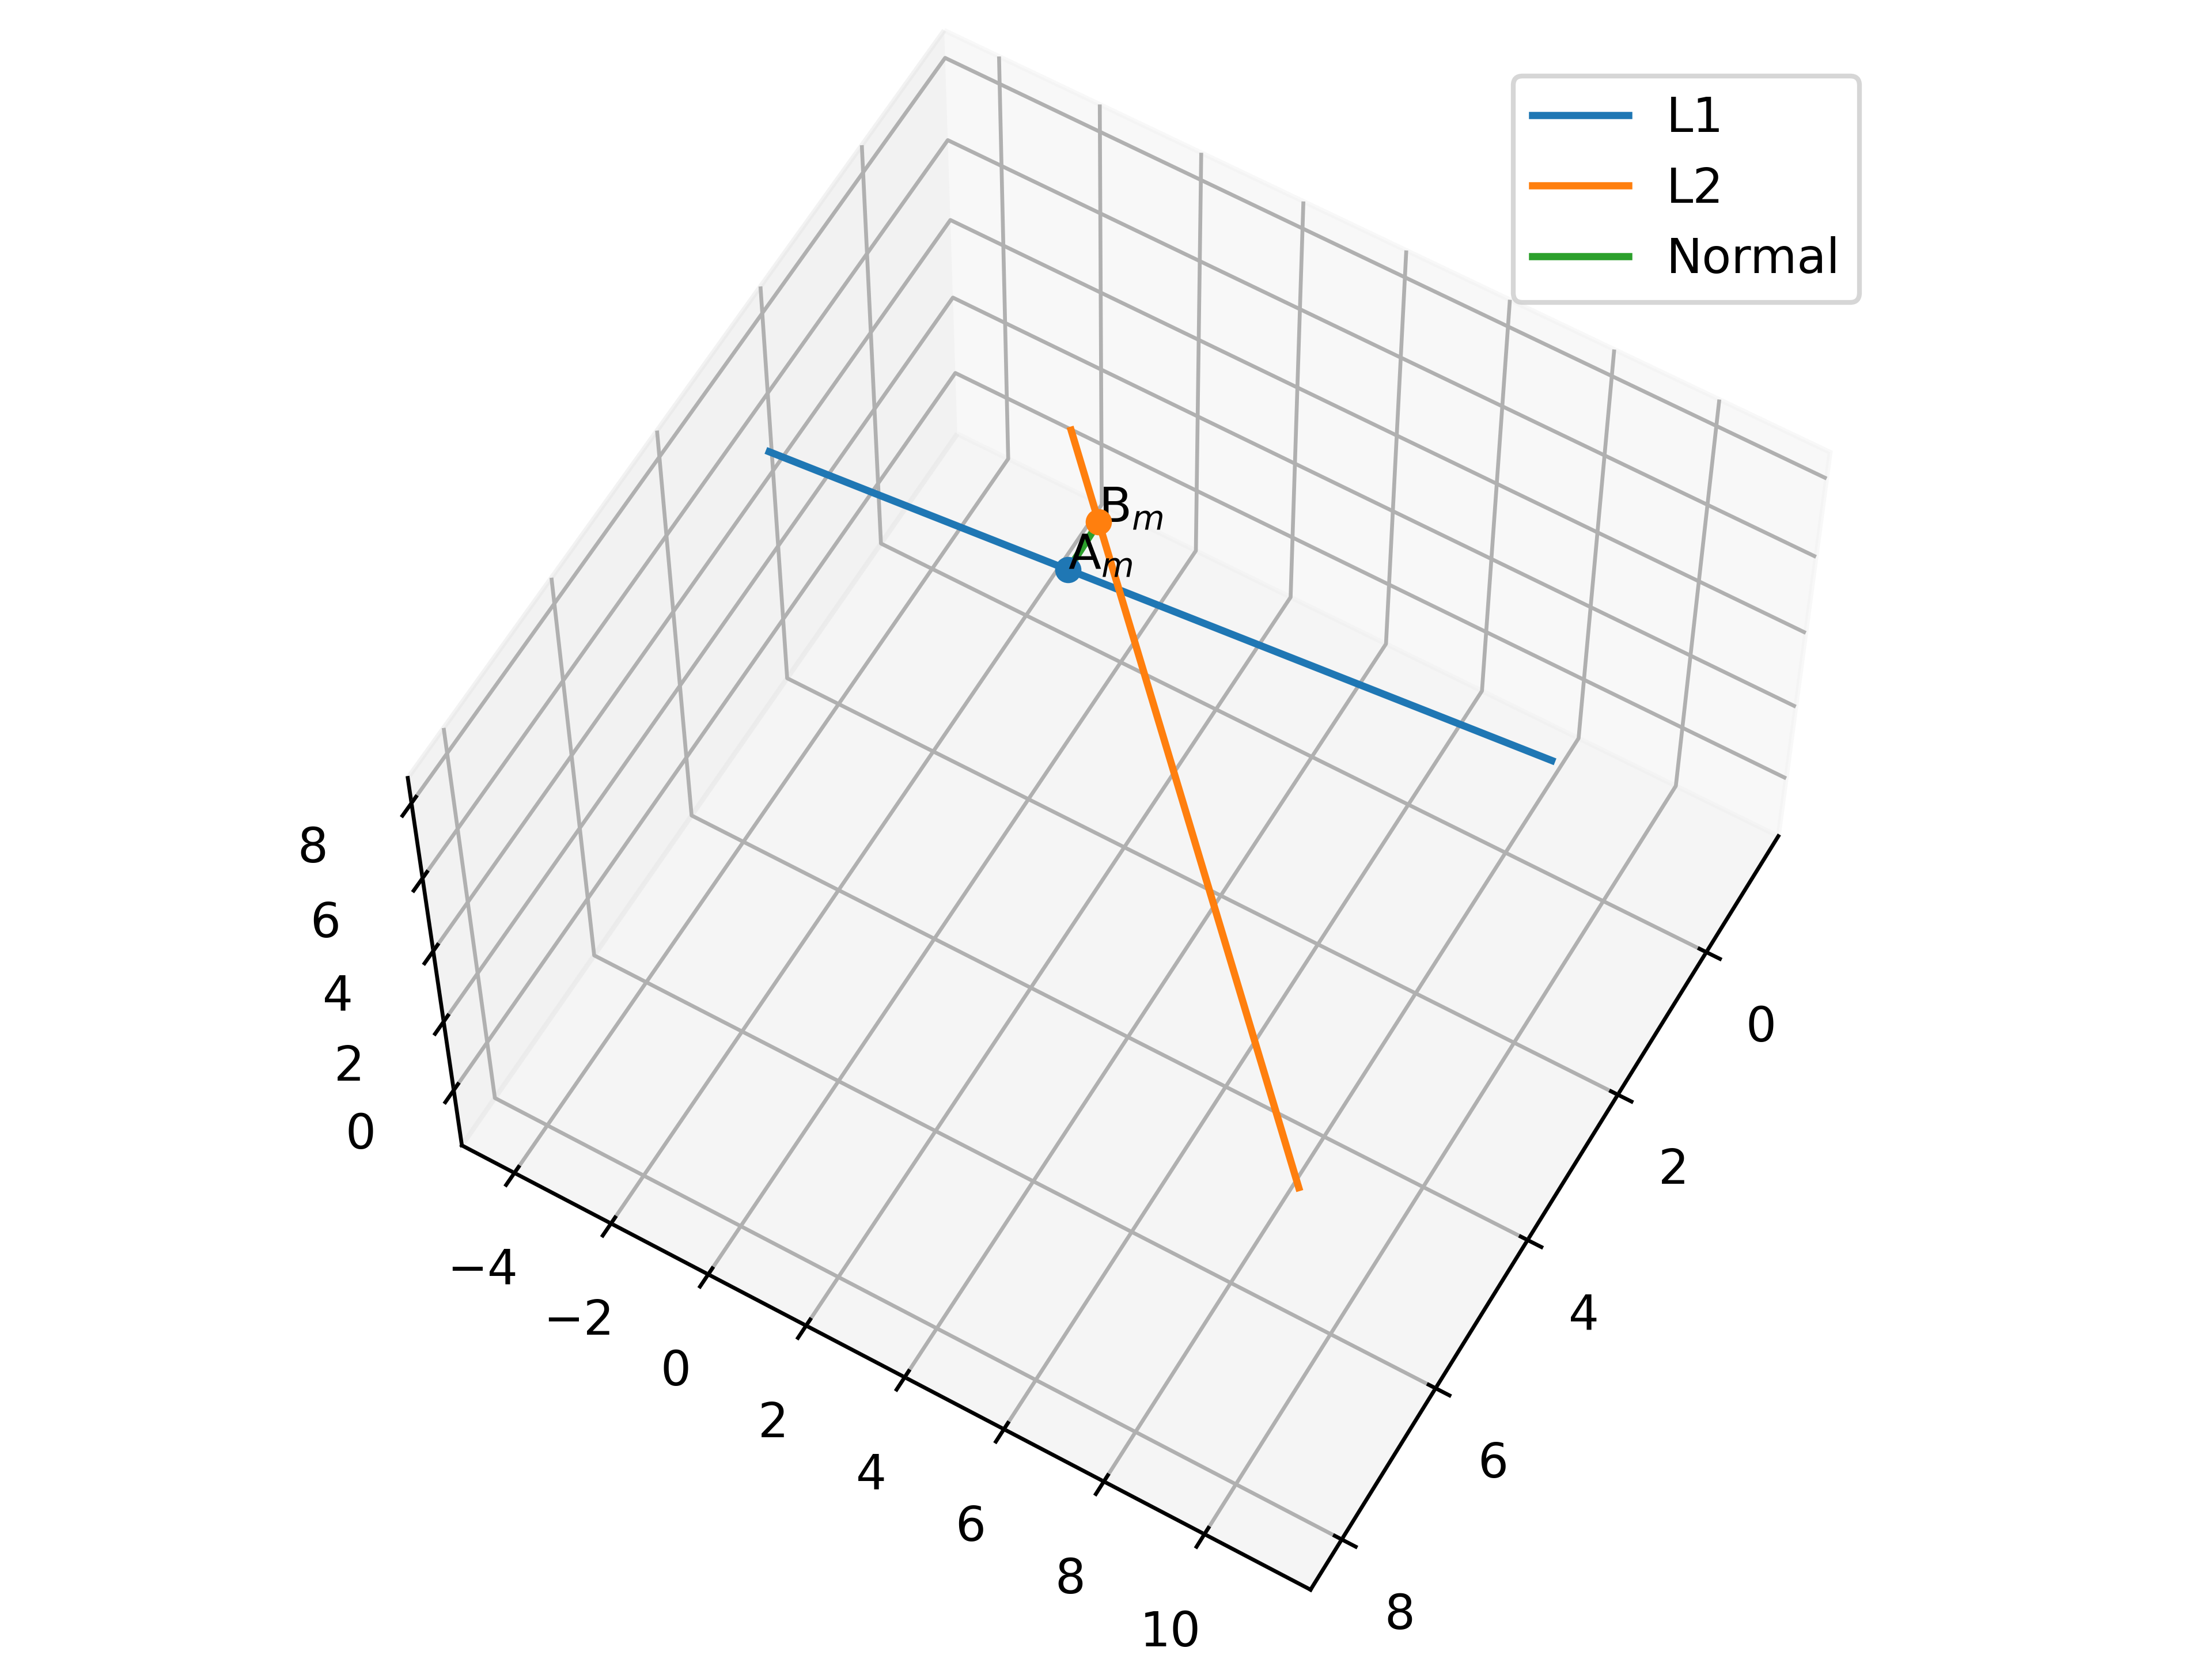
\includegraphics[width=\columnwidth]{chapters/12/11/2/16/svd/figs/skew_svd.png}
        \caption{Finding the shortest distance between two lines using SVD.}
        \label{fig:chapters/12/11/2/16/svd/svd}
    \end{figure}
